\documentclass{standalone}
\usepackage{graphicx}	
\usepackage{amssymb, amsmath}
\usepackage{color}
\usepackage{wasysym}

\usepackage{tikz}
\usetikzlibrary{intersections, backgrounds}
\usepackage{pgfmath}

\definecolor{light}{RGB}{220, 188, 188}
\definecolor{mid}{RGB}{185, 124, 124}
\definecolor{dark}{RGB}{143, 39, 39}
\definecolor{highlight}{RGB}{180, 31, 180}
\definecolor{gray10}{gray}{0.1}
\definecolor{gray20}{gray}{0.2}
\definecolor{gray30}{gray}{0.3}
\definecolor{gray40}{gray}{0.4}
\definecolor{gray60}{gray}{0.6}
\definecolor{gray70}{gray}{0.7}
\definecolor{gray80}{gray}{0.8}
\definecolor{gray90}{gray}{0.9}
\definecolor{gray95}{gray}{0.95}

\newcommand*{\offset}{0.025}

\begin{document}

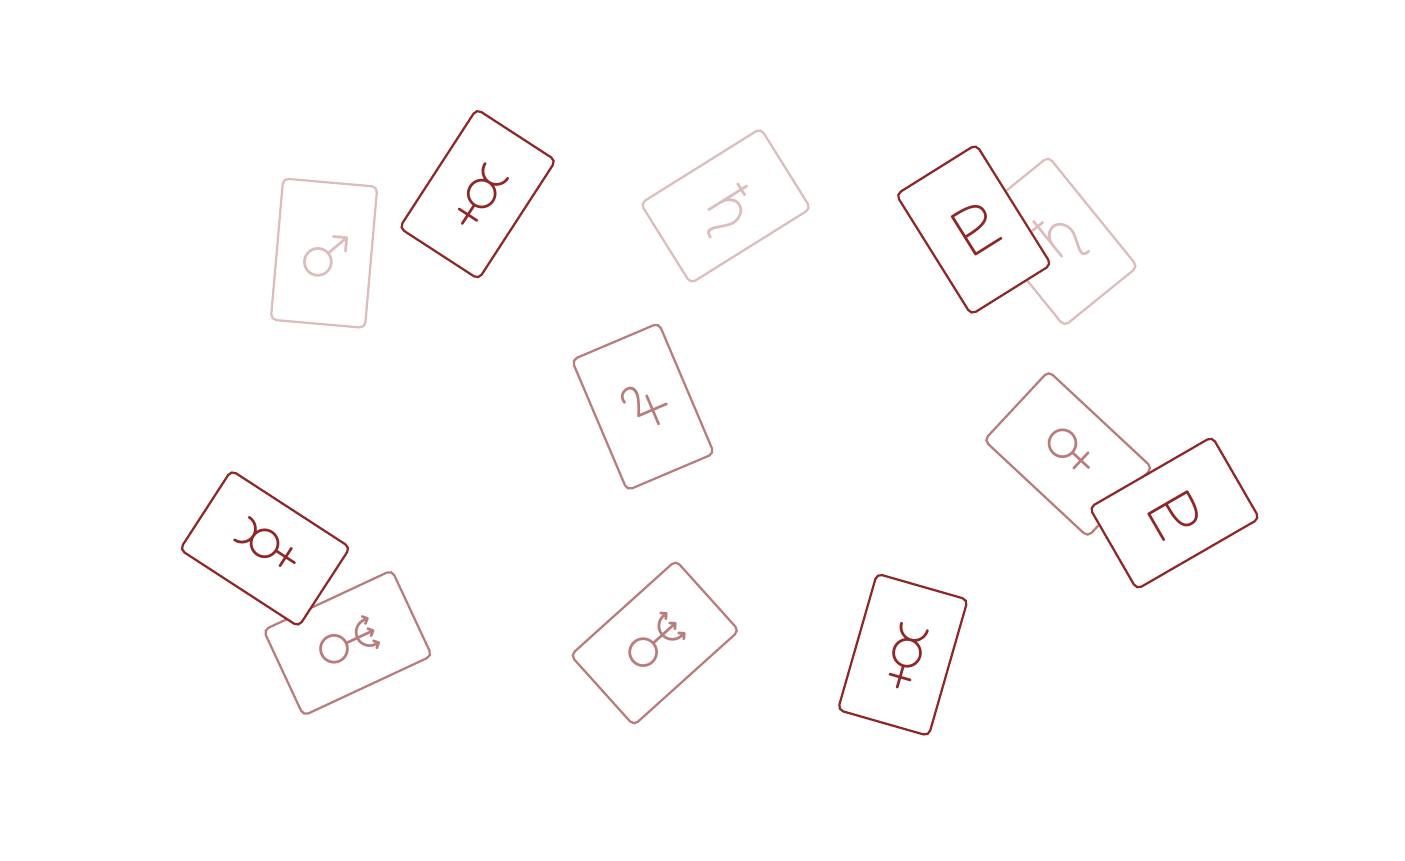
\begin{tikzpicture}[scale=0.3, thick]

\pgfmathsetmacro{\cx}{2}
\pgfmathsetmacro{\cy}{3}

\draw[white] (-28.5, -17) rectangle (28.5, 17);

% Row One
\pgfmathsetmacro{\phi}{-58}
\pgfmathsetmacro{\x}{1}
\pgfmathsetmacro{\y}{9.5}
\begin{scope}[shift={(\x, \y)}, rotate={\phi}]
  \filldraw[fill=white, draw=light, rounded corners=2] (0 - \cx, 0 - \cy) rectangle (0 + \cx, 0 + \cy);
  \node[light, rotate={\phi}] at (0.17, 0) { $\Huge \saturn$ }; 
\end{scope}

\pgfmathsetmacro{\phi}{39}
\pgfmathsetmacro{\x}{15}
\pgfmathsetmacro{\y}{8}
\begin{scope}[shift={(\x, \y)}, rotate={\phi}]
  \filldraw[fill=white, draw=light, rounded corners=2] (0 - \cx, 0 - \cy) rectangle (0 + \cx, 0 + \cy);
  \node[light, rotate={\phi}] at (0.17, 0) { $\Huge \saturn$ }; 
\end{scope}

\pgfmathsetmacro{\phi}{-5}
\pgfmathsetmacro{\x}{-16}
\pgfmathsetmacro{\y}{7.5}
\begin{scope}[shift={(\x, \y)}, rotate={\phi}]
  \filldraw[fill=white, draw=light, rounded corners=2] (0 - \cx, 0 - \cy) rectangle (0 + \cx, 0 + \cy);
  \node[light, rotate={\phi}] at (0.17, 0) { $\Huge \mars$ }; 
\end{scope}

% Row Two
\pgfmathsetmacro{\phi}{47}
\pgfmathsetmacro{\x}{15.5}
\pgfmathsetmacro{\y}{-1}
\begin{scope}[shift={(\x, \y)}, rotate={\phi}]
  \filldraw[fill=white, draw=mid, rounded corners=2] (0 - \cx, 0 - \cy) rectangle (0 + \cx, 0 + \cy);
  \node[mid, rotate={\phi}] at (0.17, 0) { $\Huge \venus$ }; 
\end{scope}

\pgfmathsetmacro{\phi}{-65}
\pgfmathsetmacro{\x}{-15}
\pgfmathsetmacro{\y}{-9}
\begin{scope}[shift={(\x, \y)}, rotate={\phi}]
  \filldraw[fill=white, draw=mid, rounded corners=2] (0 - \cx, 0 - \cy) rectangle (0 + \cx, 0 + \cy);
  \node[mid, rotate={\phi}] at (0.17, 0) { $\Huge \neptune$ }; 
\end{scope}

\pgfmathsetmacro{\phi}{-48}
\pgfmathsetmacro{\x}{-2}
\pgfmathsetmacro{\y}{-9}
\begin{scope}[shift={(\x, \y)}, rotate={\phi}]
  \filldraw[fill=white, draw=mid, rounded corners=2] (0 - \cx, 0 - \cy) rectangle (0 + \cx, 0 + \cy);
  \node[mid, rotate={\phi}] at (0.17, 0) { $\Huge \neptune$ }; 
\end{scope}

\pgfmathsetmacro{\phi}{23}
\pgfmathsetmacro{\x}{-2.5}
\pgfmathsetmacro{\y}{1}
\begin{scope}[shift={(\x, \y)}, rotate={\phi}]
  \filldraw[fill=white, draw=mid, rounded corners=2] (0 - \cx, 0 - \cy) rectangle (0 + \cx, 0 + \cy);
  \node[mid, rotate={\phi}] at (0.17, 0) { $\Huge \jupiter$ }; 
\end{scope}

% Row Three
\pgfmathsetmacro{\phi}{-33}
\pgfmathsetmacro{\x}{-9.5}
\pgfmathsetmacro{\y}{10}
\begin{scope}[shift={(\x, \y)}, rotate={\phi}]
  \filldraw[fill=white, draw=dark, rounded corners=2] (0 - \cx, 0 - \cy) rectangle (0 + \cx, 0 + \cy);
  \node[dark, rotate={\phi}] at (0.17, 0) { $\Huge \mercury$ }; 
\end{scope}

\pgfmathsetmacro{\phi}{-16}
\pgfmathsetmacro{\x}{8.5}
\pgfmathsetmacro{\y}{-9.5}
\begin{scope}[shift={(\x, \y)}, rotate={\phi}]
  \filldraw[fill=white, draw=dark, rounded corners=2] (0 - \cx, 0 - \cy) rectangle (0 + \cx, 0 + \cy);
  \node[dark, rotate={\phi}] at (0.17, 0) { $\Huge \mercury$ }; 
\end{scope}

\pgfmathsetmacro{\phi}{57}
\pgfmathsetmacro{\x}{-18.5}
\pgfmathsetmacro{\y}{-5}
\begin{scope}[shift={(\x, \y)}, rotate={\phi}]
  \filldraw[fill=white, draw=dark, rounded corners=2] (0 - \cx, 0 - \cy) rectangle (0 + \cx, 0 + \cy);
  \node[dark, rotate={\phi}] at (0.17, 0) { $\Huge \mercury$ }; 
\end{scope}

\pgfmathsetmacro{\phi}{32}
\pgfmathsetmacro{\x}{11.5}
\pgfmathsetmacro{\y}{8.5}
\begin{scope}[shift={(\x, \y)}, rotate={\phi}]
  \filldraw[fill=white, draw=dark, rounded corners=2] (0 - \cx, 0 - \cy) rectangle (0 + \cx, 0 + \cy);
  \node[dark, rotate={\phi}] at (0.17, 0) { $\Huge \pluto$ }; 
\end{scope}

\pgfmathsetmacro{\phi}{-60}
\pgfmathsetmacro{\x}{20}
\pgfmathsetmacro{\y}{-3.5}
\begin{scope}[shift={(\x, \y)}, rotate={\phi}]
  \filldraw[fill=white, draw=dark, rounded corners=2] (0 - \cx, 0 - \cy) rectangle (0 + \cx, 0 + \cy);
  \node[dark, rotate={\phi}] at (0.17, 0) { $\Huge \pluto$ }; 
\end{scope}

\end{tikzpicture}

\end{document}  